\chapter{The \textsc{StructPF} Generation Pipeline}
\label{chap:structpf}

\section{Pipeline Architecture}
\label{sec:structpf-overview}

To create a problem that triggers Productive Failure, a human designer does not write a story and choose its numbers in a single step. Instead, as documented by Kapur and Bielaczyc in their design of the Grade~7 average-speed task~\cite{kapur2012}, designing a working PF problem follows a structured sequence of four decisions.
\begin{enumerate}[leftmargin=0.7cm,itemsep=0.25em,topsep=0.3em]
    \item \textbf{Identifying prior knowledge:} The designers first inspect earlier curriculum grades to list the concepts and methods students have already been taught, such as speed and ratios from Grades~1 to~6, so that students have familiar tools to start the problem (Requirement~1 in Section~\ref{sec:intro-motivation}).
    \item \textbf{Designing the problem structure:} Next, they choose a problem situation around the critical features of the target concept and anticipate the specific methods students will try using their prior knowledge.
    \item \textbf{Testing and adjusting the numbers:} They then test candidate numbers in pilot sessions and adjust the values so that the target concept holds while familiar shortcut methods fail to give the right answer (Requirement~2).
    \item \textbf{Writing an open problem statement:} Finally, they write the student-facing story and question so that the goal and given quantities are clear, while the solution method is left open for students to invent and explain (Requirement~3).
\end{enumerate}

As we saw in Chapter~\ref{chap:oneshot}, asking an LLM to make all four decisions in a single prompt fails because the model already knows the target formula. It either chooses convenient numbers that familiar shortcuts solve immediately or coaches the student step by step toward the canonical procedure. We have therefore chosen to structure \textsc{StructPF} around the same sequence of steps that a human designer follows, because each decision targets a specific PF mechanism from Section~\ref{subsec:bg-pf-mechanisms} and requires a different kind of check. In order to prevent the model from leaking the target formula or optimizing for the grading criteria, we also keep all planning records and canonical solutions in internal design notes and withhold both the key idea and the evaluation rubric from the final task writer.

\begin{figure}[!htb]
    \centering
    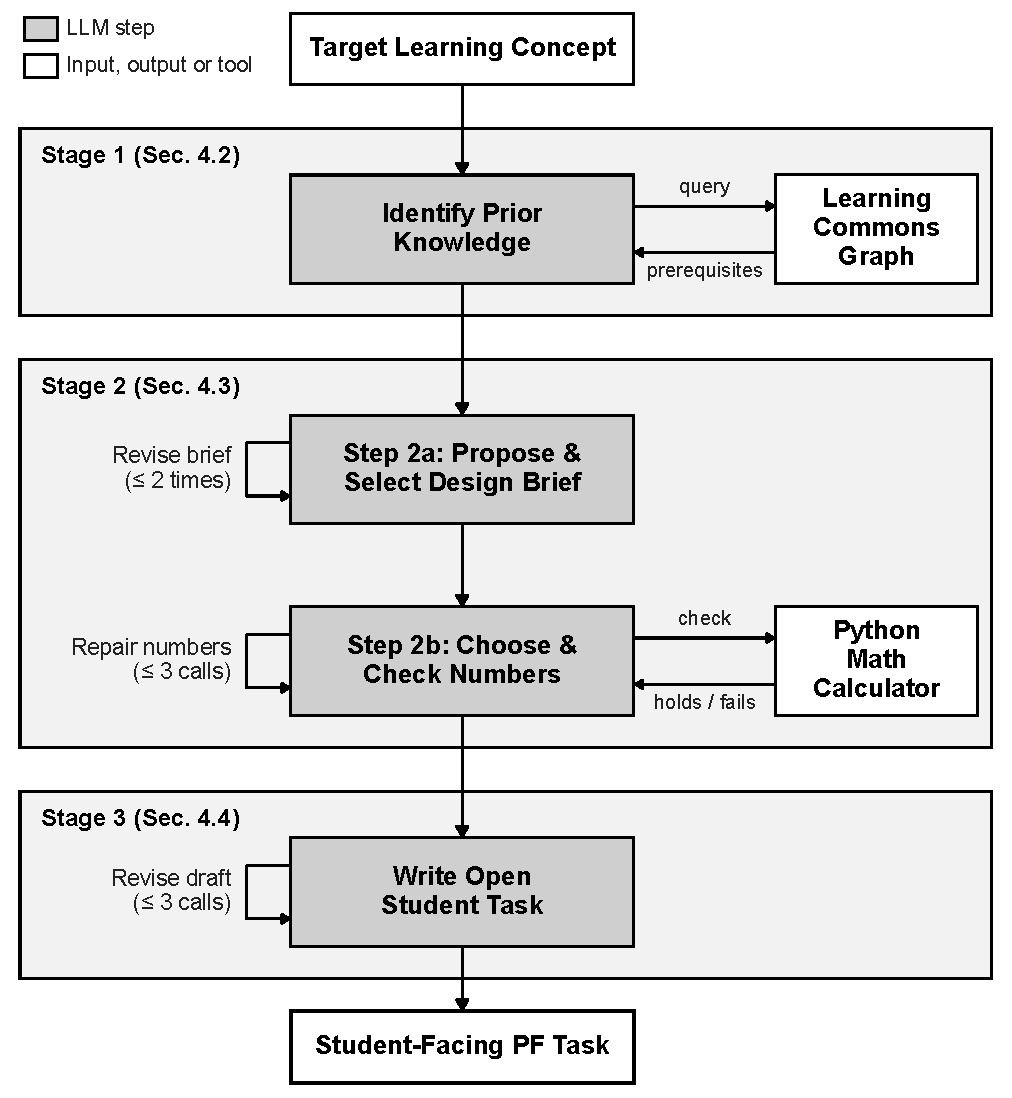
\includegraphics[width=0.56\textwidth]{figures/fig4_1_structpf_overview.pdf}
    \caption[Overview of the Three-Stage \textsc{StructPF} Pipeline]{Overview of the Three-Stage \textsc{StructPF} Pipeline}
    \label{fig:structpf-overview}
\end{figure}

Figure~\ref{fig:structpf-overview} illustrates the resulting three-stage \textsc{StructPF} pipeline, which mirrors the human design workflow and uses a fixed revision limit at each stage rather than retrying indefinitely. The following three sections introduce each stage in turn and trace the Grade~6 polygon-area standard (\texttt{6.G.A.1}) through the entire pipeline.

\section{Stage 1: Prior Knowledge Retrieval}
\label{sec:structpf-d1}

\subsection{Need for Curriculum Grounding}
\label{subsec:d1-rationale}

Stage~1 must identify the valid methods from earlier grades that students can apply before the target concept is taught. When asked directly for prerequisites, however, an LLM already knows the target concept and does not reliably separate earlier-grade skills from it, as we show in Section~\ref{sec:res-grounding}. On a Grade~8 linear-function topic, for example, prompting without curriculum data treated the two-point slope formula $(y_2 - y_1)/(x_2 - x_1)$ as already known rather than keeping the earlier proportional ratio check $y / x$, giving away the core calculation before the task was even written. Stage~1 therefore requires an external curriculum source that explicitly records which skills precede each target standard.

\subsection{The Learning Commons Knowledge Graph}
\label{subsec:d1-learning-commons}

For this curriculum source, we use the open Learning Commons Knowledge Graph (\texttt{v1.14.0})~\cite{learningcommons2025}, which connects US K--12 Common Core mathematics standards into a directed graph. As shown on the left of Figure~\ref{fig:d1-learning-commons}, the graph provides two types of links around each standard. First, \texttt{buildsTowards} links connect earlier-grade standards directly to the later-grade standard they prepare students to learn. Second, \texttt{supports} links break each standard down into smaller skills that state what a student can actually calculate. Together, these two links tell Stage~1 both which earlier standards are allowed and which concrete calculations students can try at the start of a problem.

\begin{figure}[!htb]
    \centering
    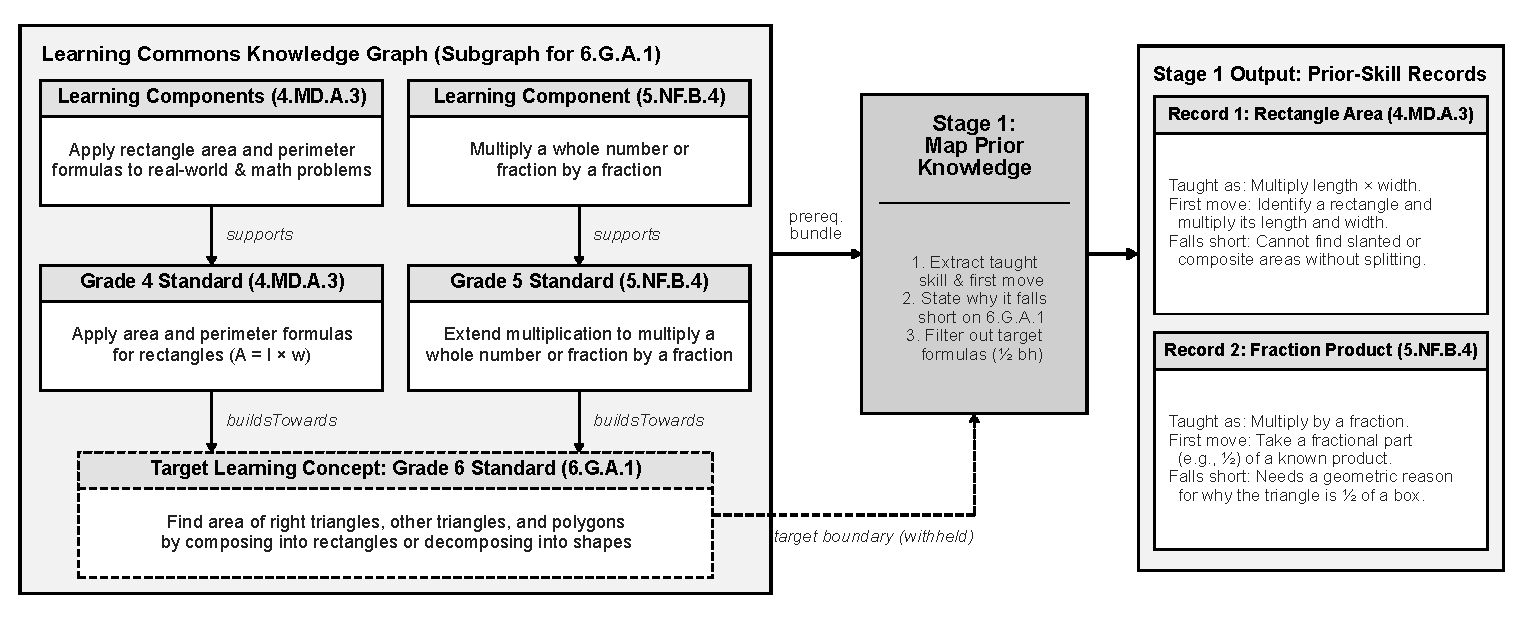
\includegraphics[width=\textwidth]{figures/fig4_2_learning_commons_graph.pdf}
    \caption[Stage 1: Prior Knowledge Retrieval for Grade 6 Polygon Area]{Stage~1: Prior Knowledge Retrieval for Grade~6 Polygon Area}
    \label{fig:d1-learning-commons}
\end{figure}

\subsection{Mapping Graph Nodes to Prior Skills}
\label{subsec:d1-extraction}

An illustration of the Stage~1 process is shown in Figure~\ref{fig:d1-learning-commons}. Given a target Common Core standard, the pipeline follows incoming \texttt{buildsTowards} edges one hop backward to retrieve its direct prerequisite standards and their attached \texttt{supports} learning components, averaging $2.6$ parent standards per target across our 30 benchmark topics. We stop at one hop because deeper traversals reach basic elementary arithmetic that is too general to design a focused PF problem. However, raw curriculum nodes only state a general skill, such as Grade~4 rectangle area, without explaining how a student would try to use it on the new topic or why it fails. Stage~1 therefore passes the retrieved prerequisite nodes and the target topic boundary to an LLM, which turns each node into a structured prior-skill record as shown on the right of Figure~\ref{fig:d1-learning-commons}. Each record states how the skill was taught in earlier grades, the initial calculation a student can try, and why that calculation falls short without the target concept. For example, on Grade~6 polygon area, the model turns Grade~4 rectangle area into multiplying length by width as a first move that cannot find slanted or composite areas without splitting, while any candidate that already uses the Grade~6 triangle formula $\frac{1}{2}bh$ is filtered out.

When a topic is given only as free text or comes from a curriculum outside US Common Core, such as Singapore Grade~7 average speed or German Grade~10 variance, Stage~1 queries the Learning Commons search API with the topic phrase to select the closest matching standards, such as Common Core unit-rate standards. If the graph has no close progression link for the level, as in undergraduate fair division, the pipeline instead retrieves grade-filtered excerpts from local curriculum documents or accepts teacher-supplied prerequisite skills.

\section{Stage 2: Problem Design and Number Verification}
\label{sec:structpf-d2}

\subsection{Step 2a: Design Brief Selection}
\label{subsec:d2a-brief}

Once Stage~1 has identified what students already know, Stage~2 must design a problem setup where familiar shortcuts fall short and verify its concrete numbers before the problem text is written. In Chapter~\ref{chap:oneshot}, asking an LLM to write the prompt directly caused all $30 / 30$ Home and Garden tasks to present already-split shapes that routine formulas solved immediately (Figure~\ref{fig:oneshot-impasse-example}). We therefore separate conceptual problem design (Step~2a) from number verification (Step~2b) and task writing (Stage~3), as illustrated for Grade~6 polygon area (\texttt{6.G.A.1}) in Figure~\ref{fig:d2-design-and-check}.

\begin{figure}[!htb]
    \centering
    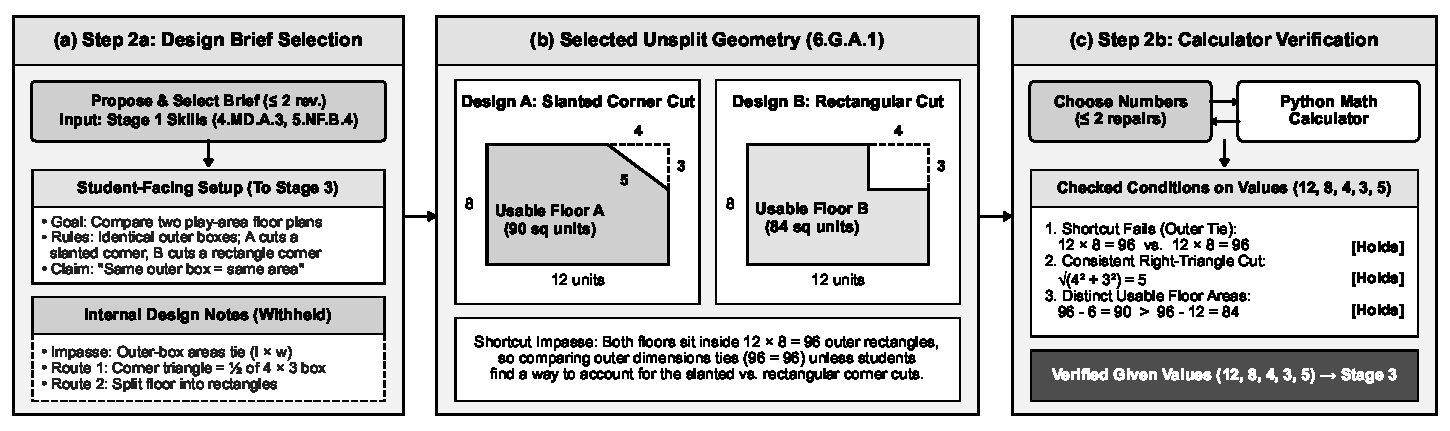
\includegraphics[width=\textwidth]{figures/fig4_3_stage2_design_and_check.pdf}
    \caption[Stage 2: Design Brief Selection (a--b) and Number Verification (c) for Grade 6 Polygon Area]{Stage~2: Design Brief Selection~(a--b) and Number Verification~(c) for Grade~6 Polygon Area}
    \label{fig:d2-design-and-check}
\end{figure}

Given the Stage~1 prior-skill records, Step~2a generates three independent candidate design briefs (prompts in Tables~\ref{tab:app-structpf-2a-propose}--\ref{tab:app-structpf-2a-translate}) so the pipeline can compare alternative problem structures before choosing numbers. As shown in Figure~\ref{fig:d2-design-and-check}a--b, each candidate brief separates the student-facing setup and open question from the withheld internal design notes that record the target key idea, the naive shortcut, and the numerical requirements. A selector model then chooses the candidate that is accessible with Stage~1 skills, causes the simplest Stage~1 shortcut to fall short, and avoids method giveaways in the student-facing fields, returning at most two revision calls if a concern remains before passing the brief to Step~2b.

\subsection{Step 2b: Task Number Verification}
\label{subsec:d2b-numbers}

To turn the selected design brief into a working problem, we need to choose concrete numbers for the quantities in the task. The goal is to ensure that the familiar shortcut fails while the geometry and the intended solution remain valid. We have chosen to use a Python calculator for this step because an LLM often picks numbers where a shortcut already works or introduces impossible dimensions when writing a problem directly (Figure~\ref{fig:oneshot-math-error-example}). For this sub-process we use \texttt{SymPy}~\cite{meurer2017sympy} to evaluate arithmetic, square roots, list totals, and equalities or inequalities. In order to keep the final answer out of the student task, we also label each number as either a student-visible given value or a withheld internal value.

An illustration of this verification process is shown in Figure~\ref{fig:d2-design-and-check}c. Every selected design brief undergoes this process (prompts summarized in Tables~\ref{tab:app-structpf-2b-propose}--\ref{tab:app-structpf-2b-repair}), which has two parts. In the first part, the model proposes concrete numbers for the quantities in the brief and separates the brief's requirements into computable conditions and qualitative rules. Only the computable conditions are translated into mathematical expressions for the calculator, whereas qualitative rules, such as keeping a figure unsplit, are checked directly against the brief. The second part of the process entails verifying the computable conditions in the Python calculator. If any condition is not satisfied, the calculator returns the computed values and the failed check to the model so that the numbers can be adjusted, repeating this step for at most two repair rounds. Finally, once all conditions hold, the verified student-visible values are passed to Stage~3, as illustrated for the play-area floor task in Table~\ref{tab:d2b-number-regimes}.

\begin{table}[!htb]
\centering
\caption[Step 2b Calculator Repair Loop for Grade 6 Polygon Area]{Step~2b Calculator Repair Loop for Grade~6 Polygon Area}
\label{tab:d2b-number-regimes}
\footnotesize
\setlength{\tabcolsep}{4.5pt}
\renewcommand{\arraystretch}{1.18}
\begin{tabular}{@{} >{\raggedright\arraybackslash}p{0.16\textwidth} >{\raggedright\arraybackslash}p{0.27\textwidth} >{\raggedright\arraybackslash}p{0.27\textwidth} >{\raggedright\arraybackslash}p{0.24\textwidth} @{}}
\toprule
\textbf{Loop Step} & \textbf{Proposed Dimensions} & \textbf{Calculator Check Result} & \textbf{Loop Action} \\
\midrule
Initial proposal & Outer boxes $12 \times 8$ vs.\ $10 \times 8$; Design~A cut $4, 3, 6$; Design~B cut $4 \times 3$ & \textbf{Rejected:} Condition~1 fails ($96 \neq 80$, outer shortcut works) and Condition~2 fails ($\sqrt{4^2+3^2} = 5 \neq 6$) & Return both failed predicates and computed values for Repair~1 \\
Repair 1 & Outer boxes both $12 \times 8$; Design~A cut $4, 3, 6$; Design~B cut $4 \times 3$ & \textbf{Rejected:} Condition~1 holds ($96 = 96$), but Condition~2 still fails ($\sqrt{4^2+3^2} = 5 \neq 6$, impossible triangle) & Return failed hypotenuse check for Repair~2 \\
Repair 2 (Final) & Outer boxes both $12 \times 8$; Design~A cut $4, 3, 5$; Design~B cut $4 \times 3$ & \textbf{Accepted:} Conditions 1--3 hold ($96 = 96$, $\sqrt{4^2+3^2}=5$, and floor areas $90 > 84$) & Freeze and pass student-visible values ($12, 8, 4, 3, 5$) to Stage~3 \\
\bottomrule
\end{tabular}
\end{table}

\section{Stage 3: Open Task Writing}
\label{sec:structpf-d3}

To complete the task design, we need to turn the verified problem setup and numbers from Stage~2 into a clear student-facing problem while leaving the solution method open for students to invent. The Stage~3 writer prompt is summarized in Table~\ref{tab:app-structpf-3-write}. As we saw in Chapter~\ref{chap:oneshot}, when an LLM sees the target concept and the five-dimension evaluation rubric while writing the task, it frequently coaches the student by naming specific representations or breaking the problem into a step-by-step worksheet (Figure~\ref{fig:oneshot-giveaway-example}). We have therefore chosen to place an information barrier between Stage~2 and Stage~3, because a language model that sees the canonical solution or the grading rubric when writing the task turns internal planning notes into student hints.

\begin{figure}[!htb]
    \centering
    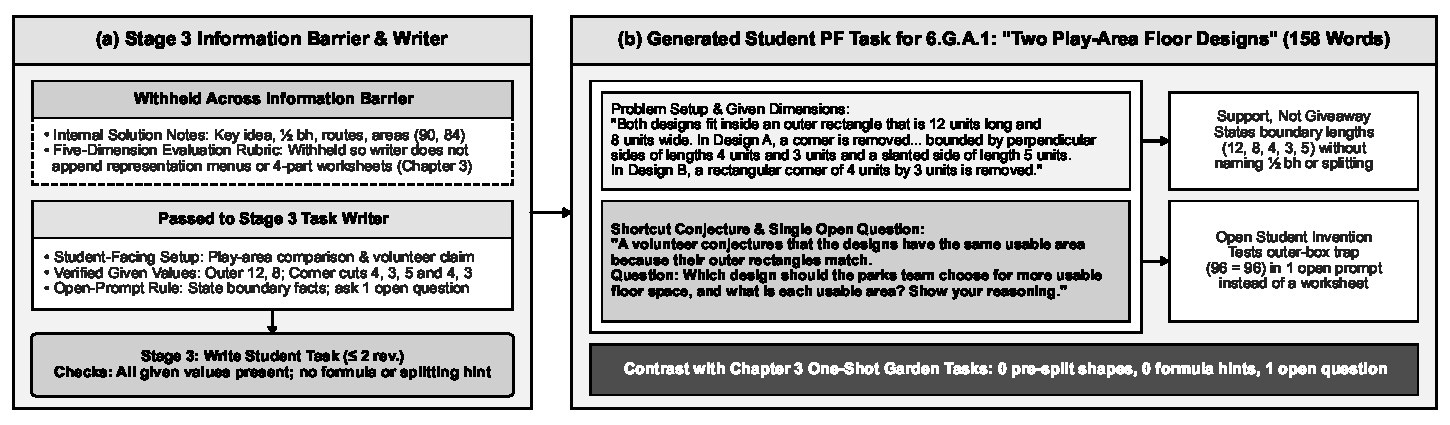
\includegraphics[width=\textwidth]{figures/fig4_4_stage3_task_writer.pdf}
    \caption[Stage 3: Information Barrier and Student-Facing Task for Grade 6 Polygon Area]{Stage~3: Information Barrier and Student-Facing Task for Grade~6 Polygon Area}
    \label{fig:d3-task-writer}
\end{figure}

An illustration of Stage~3 and the resulting task for our Grade~6 polygon-area example is shown in Figure~\ref{fig:d3-task-writer}. Passing only the student-facing setup and the verified student-visible numbers across the barrier produces a concise task (\emph{``Two Play-Area Floor Designs''}) that defines the comparison clearly while keeping the polygons unsplit and leaving the solution strategy to the student.

By separating prior knowledge retrieval (Stage~1), problem design and number verification (Stage~2), and open task writing (Stage~3), \textsc{StructPF} mirrors the four decisions of a human PF designer while keeping internal planning notes and evaluation rubrics out of the student-facing prompt. To test whether the generated tasks actually resist familiar shortcuts and elicit multiple student approaches, Chapter~\ref{chap:eval-framework} introduces \textsc{PF Eval}.

